% !TEX root = Master.tex

In Section \ref{ssec:data_sources} we introduced the setup of the data to be treated. As one can see in \autoref{tab:article_master_data}, each article can be assigned to a set of attributes. Besides some elemental attributes like \textit{color}, \textit{age group} or \textit{gender}, the data exhibit a "natural" company-specific hierarchical structure. In \autoref{fig:article_hierarchy}, we can see an example of such a hierarchy for the attributes \textit{business unit} and \textit{product division}. The bottom level consists of the articles themselves and at the top level we have the brand. Note that the brand \textit{Reebok} also belongs to adidas-group, but we are only concerned with adidas products within the scope of this thesis. 

\begin{figure}[H]
\centering
  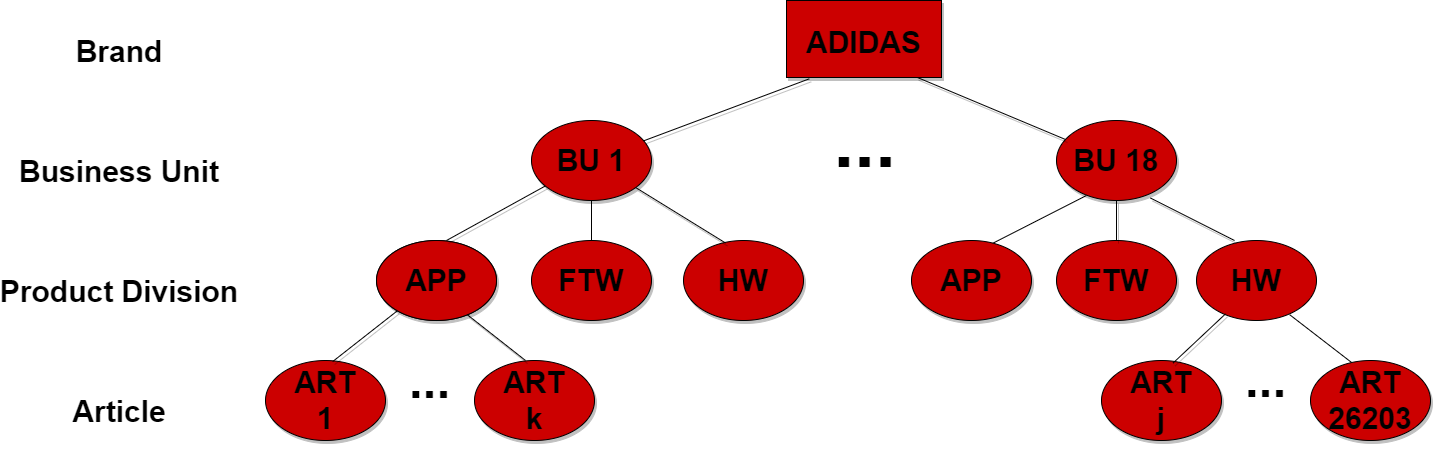
\includegraphics[width=.95\linewidth]{figures/article_tree_white.png}
  \caption{Illustration of the article's hierarchical structure using only a fraction of attributes: brand, business unit, product division (APP: Apparel, FTW: Footwear, HW: Hardware), articles.}
  \label{fig:article_hierarchy}
\end{figure}






